\subsubsection{\stid{4.13} ECP/VTK-m}

\paragraph{Overview}
As exascale simulations generate data, scientists must extract information and understand their results.
One of the primary mechanisms for understanding these results is producing visualizations that can be viewed and manipulated.
The VTK-m project is developing and deploying a scientific visualization library for exascale machines.
This library can be used directly by simulation codes or by other visualization products, and VTK-m is embedded in other Exascale Computing Project (ECP) solutions and is the sole project providing support for exascale architectures.
VTK-m supports features such as the shared-memory parallelism available on many-core CPUs and GPUs by redeveloping, implementing, and supporting necessary visualization algorithms.

One of the biggest recent changes in high-performance computing is the increasing use of accelerators.
Accelerators contain processing cores that independently are inferior to a core in a typical CPU, but these cores are replicated and grouped so that their aggregate execution provides a very high computation rate at a much lower power.
Current and future CPU processors also require much more explicit parallelism.
Each successive version of the hardware packs more cores into each processor, and technologies such as hyperthreading and vector operations require even more parallel processing to leverage each core’s full potential.

The VTK-m team is providing general-purpose scientific visualization software for exascale architectures that supports shared memory parallelism and fine-grained concurrency.
The team is focused on providing abstract models for data and execution that can be applied to a variety of algorithms across many different processor architectures along with necessary visualization algorithm implementations.
The results of this project will be delivered in tools currently used around the world today, such as ParaView and VisIt, as well as in new tools, such as Ascent, and in a stand-alone form.

\paragraph{Key Challenges}
The scientific visualization research community has been building scalable HPC algorithms for over 20 years, and today there are multiple production tools that provide excellent scalability.
However, our current visualization tools are based on a message-passing programming model.
More to the point, they rely on a coarse decomposition with ghost regions to isolate parallel execution \cite{Ahrens2001,Childs2010}.
However, this decomposition works best when each processing element has on the order of a hundred thousand to a million data cells \cite{ParaViewTutorial} and is known to break down as we approach the level of concurrency needed on modern accelerators \cite{Moreland2012:Ultravis,Moreland2013:UltraVis}.

The VTK-m project addresses this challenge by providing the core capabilities to perform scientific visualization on exascale architectures, which can then be used within current tools, used by new libraries for in situ processing, or used directly by simulation codes.
This fills the critical feature gap of performing efficient visualization and analysis on many-core CPU and GPU architectures.


\paragraph{Solution Strategy}
The ECP/VTK-m project leverages VTK-m \cite{Moreland2016:VTKm} to overcome these key challenges.
VTK-m has a software framework that provides the following critical features.

\begin{enumerate}
\item \textbf{Visualization building blocks:}
  VTK-m contains the common data structures and operations required for scientific visualization.
  This base framework simplifies the development of visualization algorithms \cite{VTKmUsersGuide}.
\item \textbf{Device portability:}
  VTK-m uses the notion of an abstract device adapter, which allows algorithms written once in VTK-m to run well on many computing architectures.
  The device adapter is constructed from a small but versatile set of data parallel primitives, which can be optimized for each platform \cite{Blelloch1990}.
  It has been shown that this approach not only simplifies parallel implementations, but also allows them to work well across many platforms \cite{Lo2012,Larsen2015,Moreland2015} and while still providing performance comparable to less portable solutions \cite{Moreland2021}.
  Within the device adapter we are leveraging Kokkos \cite{Edwards2011} to rapidly port to ECP hardware.
\item \textbf{Flexible integration:}
  VTK-m is designed to integrate well with other software.
  This is achieved with flexible data models to capture the structure of applications' data \cite{Meredith2012} and array wrappers that can adapt to target memory layouts \cite{Moreland2012:PDAC}.
\end{enumerate}


\begin{figure}[t]
  \centering

  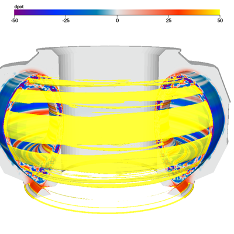
\includegraphics[height=1.35in]{projects/2.3.4-DataViz/2.3.4.13-ECP-VTK-m/VTKm-wdm-in-situ.png}\quad
  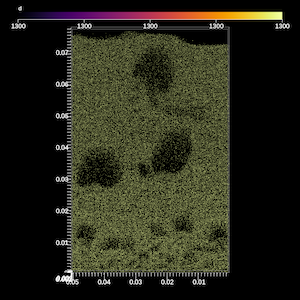
\includegraphics[height=1.35in]{projects/2.3.4-DataViz/2.3.4.13-ECP-VTK-m/VTKm-particle-spheres.png}%
  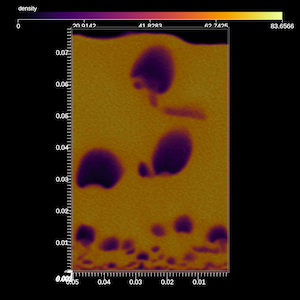
\includegraphics[height=1.35in]{projects/2.3.4-DataViz/2.3.4.13-ECP-VTK-m/VTKm-particle-density.png}\quad
  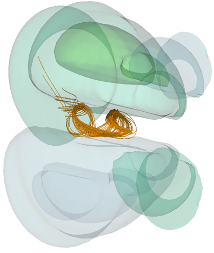
\includegraphics[height=1.35in]{projects/2.3.4-DataViz/2.3.4.13-ECP-VTK-m/VTKm-warpx-flow.png}\quad
  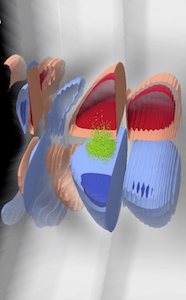
\includegraphics[height=1.35in]{projects/2.3.4-DataViz/2.3.4.13-ECP-VTK-m/VTKm-warpx-in-situ.png}\quad
  \caption{
    Examples of recent progress in VTK-m include (from left to right) in situ visualization with WDMApp simulations, particle density estimation, flow in laser wakefields, and in situ visualization with WarpX simulations.
  }
  \label{fig:VTKmRecent}
\end{figure}

\paragraph{Recent Progress}
The VTK-m project is organized into many implementation activities.
The following features have been completed in the FY20 fiscal year.

\begin{itemize}
\item \textbf{VTK-m Releases:}
  VTK-m 1.6 was released in May 2021.
\item \textbf{Kokkos:}
  Device adapters in VTK-m can now leverage the Kokkos programming model to more rapidly port to ECP hardware.
\item \textbf{WDMApp:}
  Using specialized data adapters, VTK-m is able to link into the code coupling framework used by WDMApp to provide real-time in situ visualization as demonstrated in Figure \ref{fig:VTKmRecent}.
\item \textbf{Lagrangian Basis Flows:}
  By integrating VTK-m's particle advection code, the VTK-m and ALPINE teams demonstrated high performance with significant data reduction by computing lagrangian basis flows for subsequent flow visualization \cite{Sane2021:EGPGV,Sane2021:ICCS}.
\item \textbf{Particle Density Estimation:}
  Finding structures like bubbles in mesh-free data requires estimating the density of free-floating particles. VTK-m can now quickly estimate the density distribution of particles over a volume as demonstrated in Figure \ref{fig:VTKmRecent}.
\item \textbf{Laser Wakefield Flow:}
  Particles in a laser wakefield move with physics particular to the electromagnetic fields. VTK-m's flow visualization is customized to properly compute particle paths in laser wakefield simulations from WarpX as shown in Figure \ref{fig:VTKmRecent}.
\item \textbf{WarpX:}
  As the underlying implementation of geometry processing and rendering in Ascent, VTK-m provides in situ visualization to WarpX simulations as shown in Figure \ref{fig:VTKmRecent}.
\end{itemize}

\paragraph{Preliminary Experiences on Early Access systems}
The ECP/VTK-m team has made significant progress toward supporting visualization on the Spock early access system for Frontier during FY21.
At the beginning of FY21, the team could compile a VTK-m smoke test with HIP and run it on an AMD GPU.
This demonstrated running a VTK-m ``worklet'' (the encapsulation of a GPU kernel) on the GPU.
This required resolving lots of special templating within the VTK-m software and was an achievement in its own right.

However, at the beginning of FY21, most of the features of VTK-m had to be disabled.
This included mesh structures, filtering, and rendering, which comprises the major functionality implemented within the toolkit.
FY21 included a major overhaul of the problematic features that were preventing operation on AMD hardware.
The biggest change was the removal of virtual methods.
VTK-m's use of virtual methods was problematic for all GPU types and some required features were not supported on AMD.
The removal of virtual methods required careful consideration of compiled data types that could no longer be hidden behind virtual method interfaces.
New techniques to reduce template code paths needed to be designed.
Another big overhaul was in the classes managing arrays.
Array handles were redesigned to use buffer management of un-typed arrays.
This moved much of the array management into libraries where they did not have to be recompiled for every use of every type.
It also provided some more efficient ways to manage the allocation and transfer of data.

In addition to these internal changes, the VTK-m team worked closely with the Kokkos team and had regular meetings with AMD engineers.
Progress required changes to VTK-m, Kokkos, HIP, and compilers.
Here is a selection of links to software updates that were required.

\begin{itemize}
  \setlength{\itemsep}{0pt}
  \setlength{\parskip}{0pt}
  \setlength{\parsep}{0pt}
\item\url{https://github.com/kokkos/kokkos/issues/3431}
\item\url{https://gitlab.kitware.com/vtk/vtk-m/-/merge_requests/2282}
\item\url{https://gitlab.kitware.com/vtk/vtk-m/-/merge_requests/2276}
\item\url{https://github.com/ROCm-Developer-Tools/HIP/pull/2183}
\item\url{https://github.com/spack/spack/pull/19816}
\item\url{https://github.com/kokkos/kokkos/issues/3581}
\item\url{https://github.com/kokkos/kokkos/pull/3953}
\item\url{https://gitlab.kitware.com/cjy7117/vtk-m/-/tree/hip-support}
\item\url{https://reviews.llvm.org/D112733}
\end{itemize}

Currently, VTK-m with its test suite can be compiled on Spock.
There are some caveats, however.
It requires a ROCm 5.0 pre-release and the latest head of Kokkos.
There is also currently an issue with linking the rendering library, which is being looked into.

\begin{figure}[ht]
  \centering
  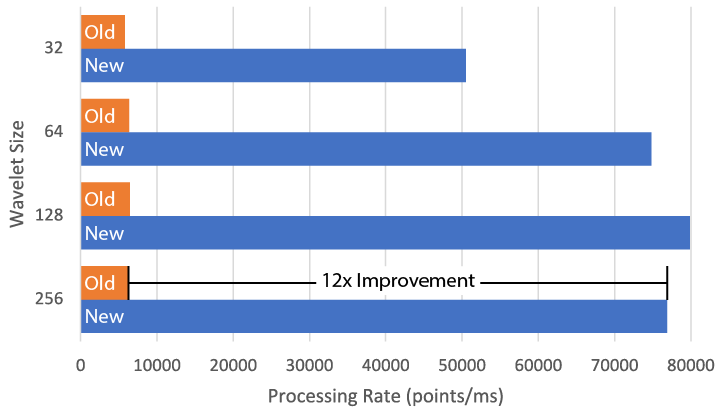
\includegraphics[width=3in]{projects/2.3.4-DataViz/2.3.4.13-ECP-VTK-m/VTKm-spock-timing.png}
  \caption{Performance improvement of VTK-m's unstructured gradient benchmark under Kokkos.}
  \label{fig:VTKmPerf}
\end{figure}

The VTK-m team has also been working with the Kokkos team to improve performance while using Kokkos to drive devices, which is necessary for AMD GPUs.
During this time, a performance issue for estimating gradients in unstructured grids was found.
The VTK-m and Kokkos teams worked together to identify a register spilling problem in one of the GPU kernels.
The kernel launch parameters for this case, and a 12-fold improvement for this algorithm was observed on Spock.

\paragraph{Next Steps}
The VTK-m team is focused on ensuring success with our KPP-3 metric.
To ensure this, our next efforts include:

\begin{itemize}
\item \textbf{Satisfy Needs of ECP Applications:}
  The VTK-m team's KPP-3 milestones hinge on applications using VTK-m code in a useful way.
  To ensure that VTK-m is satisfying the needs of ECP applications, the team will making modifications as needed.
  The initial focus will be with the WarpX, WDMApp, MFiX-Exa, and Nyx applications.
\item \textbf{Porting to Exascale Architecture:}
  As Frontier becomes available, the VTK-m team will ensure that the software compiles, runs, and performs well on the platform.
\item \textbf{Ease of Adoption:}
  The VTK-m team will address complications with integrating the VTK-m software with other software projects.
  Part of this work includes isolating external code from device code.
  Another part includes improving compile times.
\end{itemize}
